
\documentclass[12pt,a4paper]{article}
\usepackage{geometry}
 \geometry{
 a4paper,
 total={170mm,257mm},
 left=20mm,
 top=20mm,
 }
\usepackage[utf8]{inputenc}
\usepackage[T1]{fontenc}
%\geometry{verbose,tmargin=3cm,bmargin=2cm,lmargin=2cm,rmargin=2cm,headheight=2cm,headsep=2cm,footskip=2cm}
\usepackage{array}
\usepackage{float}
\usepackage{textcomp}
\usepackage{slashed}
\usepackage{amsmath}
\usepackage{graphicx}

\makeatletter

%%%%%%%%%%%%%%%%%%%%%%%%%%%%%% LyX specific LaTeX commands.
%% Because html converters don't know tabularnewline
\providecommand{\tabularnewline}{\\}

\makeatother

\usepackage{babel}
\begin{document}

\section{Industrielektronikk}


\subsection{SI-prefikser}

I industrielektronik har vi ofte veldig store eller små størrelser. Det
kan være en Harddisk på 2TB. Eller en snakker om størrelsen på transistorene
i en prosessor som kan være 7nm

\noindent \begin{center}
	\includegraphics[width=12cm]{SIenheter.eps}
\par\end{center}

\noindent \begin{center}
\begin{tabular}{|c|c|c|}
\hline 
$10^{n}$ & Prefiks  & Symbol\tabularnewline
\hline 
\hline 
$10^{24}$ & yotta  & Y\tabularnewline
\hline 
$10^{21}$ & zetta  & Z\tabularnewline
\hline 
$10^{18}$ & exa  & E\tabularnewline
\hline 
$10^{15}$ & peta  & P\tabularnewline
\hline 
$10^{12}$ & tera  & T\tabularnewline
\hline 
$10^{9}$ & giga  & G\tabularnewline
\hline 
$10^{6}$ & mega  & M\tabularnewline
\hline 
$10^{3}$ & kilo  & k\tabularnewline
\hline 
$10^{2}$ & hekto  & h\tabularnewline
\hline 
$10^{1}$ & deka  & \tabularnewline
\hline 
 &  & \tabularnewline
\hline 
$10^{-1}$ & desi  & d\tabularnewline
\hline 
$10^{-2}$ & centi  & c\tabularnewline
\hline 
$10^{-3}$ & milli  & m\tabularnewline
\hline 
$10^{-6}$ & mikro  & \textmu{}\tabularnewline
\hline 
$10^{-9}$ & nano  & n\tabularnewline
\hline 
$10^{-12}$ & pico  & p\tabularnewline
\hline 
$10^{-15}$ & femto  & f\tabularnewline
\hline 
$10^{-18}$ & atto  & a\tabularnewline
\hline 
$10^{-21}$ & zepto  & z\tabularnewline
\hline 
$10^{-24}$ & yocto  & y\tabularnewline
\hline 
\end{tabular}
\par\end{center}

\subsection{Atomstrukturen}

Et atom består at nøytroner, protoner og elektroner. Disse er organisert
i en kjerne bestående av nøytroner og protoner. Utenpå ligger flere
skall med elektroner. Hvert skall kan ha $2n^{2}$ elektroner, men
det ytterste kan maks ha 8 elektroner. Dette kaller vi valensskallet.
Alle atomer må ha like mange elektroner som det har protoner i kjernen.
Hvor mange det har avgjør hvilket stoff det er. 

De elektriske egenskapene til et stoff kan vi grovt dele inne tre
klasser. 
\begin{itemize}
\item Metaller. Dette er materialer som leder godt. De har 1-3 elektroner
i valensskallet. Disse er forholdsvis løst bundet til atomet. Vi sier
da at det har mange frie elektroner. 
\item Halvledere. Materialer som ikke leder like godt som metaller. Det
har noen unike egenskaper. Disse egenskapene gjør at vi kan bruke
det til å lage dioder, transistorer og CPU-er. 
\item Isolatorer. Materialer som leder dårlig. Disse brukes der vi ikke
vil at det skal gå strøm. 
\end{itemize}


\subsection{Elektrisk ladning}

Når det blir over- eller underskudd at elektroner i et stoff vil det
oppstå en elektrisk ladning. 

Et eksempel er statisk elektrisitet.

Et annet eksempel er et batteri. 

\noindent \begin{center}
\includegraphics{./1a.pdf}
\par\end{center}


\subsection{Spenning}

Som dere har sett er oppstår det en kraft mellom to forskjellige landinger.
Hvor stor denne ladningen er, angis i volt. Vi sier at spenning har
benevnelsen U og enheten V (volt). Det er spenningen som er drivkraften
i alle elektriske kretser. 

\subsection{Strøm}

Elektrisk strøm er elektroner i bevegelse (egentlig elektriske ladninger
i bevegelse). Elektronene flyter fra et sted til et annet. For at
elektronene skal forflytte seg fra et sted til et annet må de påvirkes
av en kraft. Denne kraften kalles spenning. 

Størrelsen på strømmen vil si hvor mange elektroner som passerer et
gitt punkt på et sekund. Når $6.25\cdot10^{18}$ elektroner passerer
pr.sek sier vi at det går en ampere. Strøm har betegnelsen I og enheten
A ampere 

\subsection{Resistans (R)}

Når det går strøm i et materiale, vil elektronene av og til kollidere
med atomer. De vil da miste litt av energien sin. Jo flere kollisjoner
jo mer blir strømmen av elektroner forhindret. Hvor mye strømmen blir
forhindret varierer fra materiale til materiale. Denne egenskapen
kaller vi resistans. 

Resistans har benevnelsen R og enheten $\Omega$ ohm. 

\subsection{Spenningskilde}

En spenningskilde leverer en elektrisk spenning. Spenningen kan blir
produsert ved hjelp av kjemisk energi i batteri, solenergi i solcellepanel,
mekanisk energi i en generator. 

Spenningskilder kan kobles i serie, da økes den totale spenningen.
Vi kaller det serie kobling av spenningskilder. Den totale spenningen
blir
\[
U_{total}=U_{1}+U_{2}+U_{3}+\cdots\cdots+U_{n}
\]

Det er også mulig å koble spenningskilder i parallell. 


\subsection{Enkel krets}

En enkel krets består av en spenningskilde, en vei for strømmen og
en belastning. 

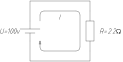
\includegraphics[width=6cm]{eksempel1.pdf}
%Tegn krets med lampe.


\subsection{Ohms lov}

I 1826 finner Georg Simon Ohm ut at spenning, strøm og resistans henger
sammen på en forutsigbar måte. Denne sammenhengen viste han med en
formel som blir kalt Ohm's lov

\begin{flalign*}
\hspace{100pt}U & =I\cdot R & \footnotesize\begin{array}{ll}
U & Spenning\,i\,V(volt)\\
I & Str\slashed{o}m\,i\,A(ampere)\\
R & Resistans\,i\,\mbox{\ensuremath{\Omega}}(ohm)
\end{array} &  & {}
\end{flalign*}

Oppgaver:
\begin{enumerate}
\item Skriv Ohm's lov med hensyn på strøm
\item Skriv Ohm's lov med hensyn på resistans
\item Skriv Ohm's lov med hensyn på spenning
\item Hvis en dobbler spenningen over en resistans minker eller øker strømmen,
og hvor mye?
\item Om en halverer spenningen over resistans, hvor mye vil strømmen endres?
\item Det er en fast spenning over en resistans, og strømmen måles til 1A.
Om en skifter ut resistansen med en på halve verdien. Hva vil da strømmen
være?
\item I en krets dobbles spenningen og resistansen halvveres. Øker eller
minker strømmen, og med hvor mye?
\item I en krets er U=2V og I=10mA. Om U forandres til 1V, hva vil strømmen
bli?
\item Hvis I=3A ved en spenning, hva vil I bli ved dobble spenningen. 
\end{enumerate}

\subsubsection{Eksempler}

\paragraph{Eksempel 1}

Hvor mange ampere går det i kretsen på figuren
\vskip 0.5cm
\begin{figure}[H]
	\begin{center}
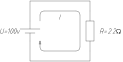
\includegraphics[width=6cm]{eksempel1.pdf}
	\end{center}
\end{figure}

\vskip 0.5cm
Løsning: Bruker formelen $I=\dfrac{U}{R}$

\[
I=\dfrac{U}{R}=\dfrac{100V}{22\Omega}=\underline{\underline{4.6A}}
\]

Lignende problem: Hva blir strømmen om R forandres til 33$\Omega$
i kretsen på figuren

\paragraph{Eksempel 2 }

Hvis resistansen i figuren forandres til 47$\Omega$ og
spenningen til 50v, hva blir strømmen?

\vskip 0.5cm
Løsning: Erstatter U=50V og R=47$\Omega$ i formelen $I=\dfrac{U}{R}$

\[
I=\dfrac{U}{R}=\dfrac{50V}{47\Omega}=\underline{\underline{1.1A}}
\]

Lignende problem: Hvis U=5V og R=1000$\Omega$, hva blir strømmen?

\paragraph{Eksempel 3}

Finn strømmen i figuren 

\vskip 0.5cm
\noindent \begin{centering}
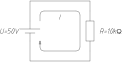
\includegraphics[width=6cm]{eksempel3.pdf}
\par\end{centering}

\vskip 0.5cm
Løsning: Husk at 1.0k$\Omega$ er det samme som $1\cdot10^{3}\Omega$.
Bruk formelen $I=\dfrac{U}{R}$

\[
I=\dfrac{U}{R}=\dfrac{50V}{1.0k\Omega}=\dfrac{50V}{1.0\cdot10^{3}}=\underline{\underline{50mA}}
\]


\paragraph{Eksempel 4}

Hvor mange milliampere går det i kretsen på figuren 

\vskip 0.5cm
\noindent \begin{centering}
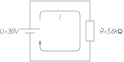
\includegraphics[width=6cm]{eksempel4.pdf}
\par\end{centering}

\vskip 0.5cm
Løsning: Bruk formelen $I=\dfrac{U}{R}$

\[
I=\dfrac{U}{R}=\dfrac{30V}{5.6k\Omega}=\dfrac{30V}{5.6\cdot10^{3}}=\underline{\underline{5.4mA}}
\]




\subsection{Seriekretser}

I en seriekrets kobles flere motstandere etter hverandre. I en slik
krets har strømmen en vei å gå. Vi kan derfor si at strømmen er den
samme overalt i en serie krets. 

Spenninen som påtrykkes seriekretsen vil fordeles seg over motstandene
etter Kirchhoff's spenningslov:
\[
U_{t}=U_{1}+U_{2}+U_{3}+......+U_{n}
\]

Eller med ord: Summen av alle spenninger i en seriekrets er null.

Total resistansen i en seriekrets finner vi ved å legge sammen alle
motstandere:
\[
R_{t}=R_{1}+R_{2}+R_{3}+......+R_{n}
\]

Tegn opp motstandere i flere mønster som skal kobles i serie.

\subsection{Parallellkretser}

I en parallellkrets er flere motstandere koblet til to punkter(noder).
Dette gjør at spenningen er lik over alle motstandere i en paralellkobling.
Stømmen igjennom en motstand i paralellkobling blir da $I=\dfrac{U}{R_{en\,eller\,annen}}$.
Summen av alle strømmer i paralellkoblingen blir det vi kaller hovedstrømmen:

\[
I_{t}=I_{1}+I_{2}+I_{3}+......+I_{n}
\]

Resisansen i en paralellkobling:

\[
R_{t}=\dfrac{1}{\dfrac{1}{R_{1}}+\dfrac{1}{R_{2}}+\dfrac{1}{R_{3}}+......+\dfrac{1}{R_{n}}}
\]


\subsection{Jord}

Med jord i elektriske kretser menes en nøytral plass. Det skal være
en plass alle strømmer skal kunne føres til bake til. Etter denne
definisjonen vil jord alltid være 0V. 

\begin{figure}[H]
\noindent \begin{centering}
\includegraphics[width=6cm]{./jord.pdf}
\par\end{centering}
\caption{Jordingspunkt i krets}
\end{figure}


\subsection{Kombinerte kretser}

Ofte finner en kretser med en kombinasjon av seriekobling og parallellkobling.
Utfordringen ligger i å finne hva som er koblet i serie og hva som
er koblet i parallell. 

\begin{figure}
\noindent \begin{centering}
\includegraphics[scale=0.9]{./kombieks1.pdf}
\par\end{centering}
\caption{\label{fig:Eksempel-p=0000E5-kombinert}Eksempel på kombinert krets}
\end{figure}

I figur \ref{fig:Eksempel-p=0000E5-kombinert} kan vi se at $R_{1}$
er i serie med parallellkoblingen av $R_{2}$ og $R_{3}$. Dette kan
vi skrive som:
\[
R_{1}+R_{2}||R_{3}
\]

Om vi vil kan vi erstatte $R_{2}||R_{3}$med en $R_{p}$. Vi har da
en serie kobling av $R_{1}+R_{p}$ 

Prøv å finne ut hvilke motstandere som er i serie og parallell i denne
kretsen:

\begin{figure}
\noindent \begin{centering}
\includegraphics[scale=0.9]{./kombieks2.pdf}
\par\end{centering}
\noindent \centering{}\caption{}
\end{figure}

Svar:
\[
R_{1}+R_{2}||R_{3}+R_{4}
\]
 
\subsection{Måling av spenning, strøm og resistans. }

\subsubsection{Måling av strøm}

For å måle strøm bruker vi et amperemeter 

\subsection{Indre resistans i spenningskilder. }

Alle spenningskilder består av det vi kan kalle en ideell spenningskilde
og en indre resistans. Ettervert som en last trekker strøm fra spenningskilden
vil spenninger over $R_{i}$ øke. Dette gjør at $U_{Ri}$ også øker.
Dette medfører at spenningen på tilkoblingspunktene synker. 
\[
U_{ut}=E-R_{i}\cdot I
\]
 

\begin{figure}[H]
\noindent \begin{centering}
\includegraphics[width=8cm]{./indreresistans.pdf}
\par\end{centering}
\caption{Spenningskilde med indre resistans}
\end{figure}


\subsection{Signal}

Når vi bruker strøm eller spenning til å overføre informasjon, kaller
vi det ofte for et signal. Et signal kan være en spenning som slås
av og på. Dette kaller vi ofte for et digitalt signal. 

Spenningen som blir sgenerert i en mikrofon kaller vi for et analogt
signal. 

\subsection{Elektriskeomponenter}

\subsubsection{Kondensatoren C{[}F{]}}

En kondensator er en elektrisk komponent som er laget for å ta i mot
ladning. Det vil si elektroner. Hvor mye lagning den kan ta imot oppgis
i Farad {[}F{]}. Farad er en gangske stor størrelse se en vil ofte
se $\mu F$ brukt. I likestrømskretser brukes den ofte til stabilisering.
I kretser med vekselstrøm (lydsignaler) brukes den i filter. For eksempel
vil en kondensator i serie med diskantelementet i en høytaler hindre
at ''bass'' frekvenser brenner opp diskanten.

Når vi kobler likestrøm til en kondensator vil den lade seg opp. Under
oppladningen vil spenningen over kondensatoren øke helt til den oppnår
tilkoblet spenning. Hvor lang tid dette har kommer an på hvor resistans
det er i kretsen. Under oppladningen vil strømmen være størst i starten
og gå mot null når kondensatoren er fult oppladet.

Vi sier at for å lade opp kondensatoren til 63\% av full ladning er
tidskonstanten til kretsen. Denne kalles $\tau$(Tau). Vi kan regne
ut denne tidskonstanten med denne formelen:
\[
\tau=RC
\]
 For at kondensatoren skal være tilnærmet fulladet må det gå 5$\tau$. 

Når vi kobler en kondensator til en vekselspenning vil den lade seg
opp når sinuskurven er på vei opp (0-90°). Så vil den lade seg ut
når sinuskurven går mot null (90-180°). Når sinuskurven synker mot
bunn (180-270°) vil kondensatoren lade seg opp med motsatt polaritet.
Og lade seg ut når sinuskurven går mot null igjen (270-360°). Når
kondensatoren skal lade seg opp og ut yter den en motstand mot strømmen.
Den motstanden kondensatoren yter kaller vi reaktans. 

Da strømmen er størst ved når vi setter spenningen på og blir mindre
etter hvert. Vil reaktansen (motstanden) til kondensatoren være avhenging
av hvor fort vekselspenningen skifter retning (frekvensen). Vi kan
regne ut reaktansen etter følgende formel: 

\[
X_{c}=\frac{1}{2\pi fC}
\]

For å gjøre regning på vekselstrøms kretser skal vi innføre en ''i''
i formelen. Vi skal ikke bry oss så mye om hva denne i-en er for noe.
Men den gjør at vi kan regne på vekselstrøms kretser som vi har gjort
med likestrømskretser. (Dette krever at vi har en kalkulator som kan
regne med i, noe som ikke er vanlig. Der for skal vi bruke www.wolframalpha.com
som kalkulator) Formelen blir da slik:

\[
X_{c}=\frac{1}{2\pi ifC}
\]

(Det er meningen at elevene skal bruke wolframalpha til å regne på
kretser med vekselspenning. Da kan det bruke ohms lov som ved DC kretser
bare en husker å bruke ''i'', wolframalpha vil da gi alle svar på
polar form.)

\begin{figure}[H]
\noindent \begin{centering}
\includegraphics[width=8cm]{./Capacitor_schematic_with_dielectric.pdf}
\par\end{centering}
\caption{Kondensator}
\end{figure}


\subsubsection{Spolen}

Litt enkelt kan vi si at en spole er en elektrisk komponent som gjør
alt den kan for å hindre en variasjon i strømmen. En hver endring
av strømmen gjennom en spole vil gi et magnetfelt i endring. Dette
magnetfeltet genererer en motsatt rettet spenning som vil hindre/begrense
strømmen. Denne effekten vil etter hvert avta. 

Når du ser en spole skal du tenke på den som en komponent som slipper
igjennom lave frekvenser (lite endring i strømmen), og som hindrer
høye frekvenser (mye endring i strømmen. )
\[
X_{L}=2\pi ifL
\]

Eksempel i simulator

\$ 1 5.0E-6 10.20027730826997 50 5.0 50

l 272 160 400 160 0 1.0 3.82582854285829E-18

r 400 160 400 288 0 100.0

v 272 288 272 160 0 0 40.0 5.0 0.0 0.0 0.5

s 272 288 400 288 0 1 false

o 0 64 0 35 5.0 0.1 0 -1

Vert å merke seg:
\begin{itemize}
\item Se på skopet. Strømmen er merket med gult og spenningen med grønt.
Er strømmen eller spenningen over spolen stor rett etter en har lagt
inn bryteren?
\end{itemize}
Oppgave

Koble en AC-voltage source til en spole i serie med en motstand. Se
på motstanden i et scope og varier frekvensen på AC kilden. Hva skjer
med spenningen over motstanden i forhold til frekvensen?

\subsubsection{Transformatoren}

Elektroniske apparater bruker skjelden/aldri spenningen i veggen direkte.
En trenger ofte en lavere spenning. Ved hjelp av en transformator
kan vi transformere ned spenningen fra 230V/AC til f.eks. 8V/AC. 

Virkemåte:

Når det går en strøm i primærviklingen dannes det et magnetfelt som
følger jernkjernen til sekundærviklingen, her induseres det en spenning.
Denne spenningen vil være lavere da sekundærviklingen har færre viklinger.
Spenningen går da fra 230V til 8V.

Forholdet mellom spenning på primærside og skundærside avgjøres av
forholdet mellom antall viklinger. Vi kan beregne dette etter følgende
formel:

\[
\frac{U_{s}}{U_{p}}=\frac{N_{s}}{N_{p}}
\]

\begin{figure}[H]
\noindent \begin{centering}
\includegraphics[width=10cm]{./Transformer.pdf}
\par\end{centering}
\caption{}
\end{figure}

Eksempel

Kode til bruk i Falstads circuit simulator:

\$ 1 5.0E-6 10.20027730826997 50 5.0 50

v 256 272 256 176 0 1 40.0 5.0 0.0 0.0 0.5

T 256 176 400 272 0 4.0 5.0 3778.7688500126737 0.028384276258977124
0.999

r 400 176 400 272 0 100.0

o 0 64 0 34 10.0 3276.8 0 -1

o 2 64 0 35 40.0 0.4 1 -1\$ 1 5.0E-6 10.20027730826997 40 5.0 50

v 256 272 256 176 0 1 8.0 5.0 0.0 0.0 0.5

T 256 176 400 272 0 4.0 5.0 -0.8567511817490633 0.1985221364880192
0.999

r 400 176 400 272 0 100.0

o 0 64 0 34 10.0 0.8 0 -1

o 2 64 0 35 40.0 0.4 0 -1

\subsubsection{Dioden}

En diode er en elektrisk komponent som leder strøm en vei. Tilkoblingspunktene
på en diode kaller vi anode og katode. Strømmen kan gå fra anoden
til katoden. Men ikke motstatt. Når strømmen går igjennom dioden vil
det legge seg ca. 0.7V over dioden, da sier ofte at dioden er i lederetning.
Når vi kobler en pluss spenning til katoden sier vi at dioden står
i sperreretning. Den vil da ikke lede noe strøm. 

\begin{figure}[H]
\noindent \begin{centering}
\includegraphics{./Diode_symbol.pdf}
\par\end{centering}
\caption{}
\end{figure}

Eksempel i Falstads circuit simulator:

\subsubsection{Likeretteren}

I elektroniske apparater har vi ofte bruk for likespenning. Når vi
driver et apparat fra batterier er ikke dette noe problem. Men vi
vil ofte bruke strømmen fra vegguttaket til å drive apparatene. Vi
må da ha en strømforsyning som kan transformere ned- og likerette
vekselspenningen. Dioden leder strøm bare en vei så denne kan vi bruke
til dette. 

Eksempel i Falstads circuit simulator:

Kode:

\$ 1 5.0E-6 10.20027730826997 50 5.0 50

d 272 176 384 176 1 0.805904783

r 384 176 384 272 0 100.0

w 272 272 384 272 0

v 272 272 272 176 0 1 40.0 5.0 0.0 0.0 0.5

o 3 64 0 34 10.0 0.025 0 -1

o 1 64 0 34 5.0 0.025 1 -1\$ 1 5.0E-6 10.20027730826997 50 5.0 50

d 272 176 384 176 1 0.805904783

r 384 176 384 272 0 100.0

w 272 272 384 272 0

v 272 272 272 176 0 1 40.0 5.0 0.0 0.0 0.5

o 3 32 0 34 9.353610478917778 0.023384026197294447 0 -1

o 1 32 0 35 5.0 0.05 0 -1

Vert å merke seg:
\begin{itemize}
\item Bare ene halvperioden av sinusspenningen blir likerettet. 
\item Spenningen over lasten ligger alltid ca 0.7V lavere. 
\item I sperrereting ligger all spenning over dioden. 
\end{itemize}

\subsubsection{LED}

\subsubsection{Fotodiode}

\subsubsection{Transistor som bryter}

\subsection{Øvingsoppgaver}
\begin{enumerate}
\item Fyll ut manglende felter\\
\begin{tabular}{|c|c|c|}
\hline 
$10^{n}$ & Prefiks  & Symbol\tabularnewline
\hline 
\hline 
$10^{12}$ & tera & \tabularnewline
\hline 
$10^{9}$ &  & G\tabularnewline
\hline 
$10^{6}$ & mega & \tabularnewline
\hline 
 & kilo  & k\tabularnewline
\hline 
 & milli  & \tabularnewline
\hline 
$10^{-6}$ & mikro  & \textmu{}\tabularnewline
\hline 
$10^{-9}$ &  & n\tabularnewline
\hline 
 & pico  & p\tabularnewline
\hline 
\end{tabular}
\item Hvor mange elektroner kan det være i valensskallet?
\item Hvor mange elektroner kan det være i valensskallet til:

\begin{enumerate}
\item Ledere
\item Halvledere 
\item Isolaorer 
\end{enumerate}
\item Hva vil det si at et stoff har elektrisk ladning?
\item Hva er benevnelsen og enheten til spenning?
\item Hva er benevnelsen og enheten til strøm?
\item Hva er benevnelsen og enheten til resistans?
\item Hva er det som gjør at et materiale har resistans?
\item Tegn symbolet for en resistor (motstand).
\item Nevn tre måter å produsere elektrisk spenning på. 
\item Hva oppnår vi ved å parallellkoble to batterier?
\item Hva oppnår vi ved å seriekoble to batterier?
\end{enumerate}

\subsubsection{Ohms lov}

I oppgave 3-13 må du tegne kretsen. 
\begin{enumerate}
\item Ohms lov skrives 
\item Vis hvordan den kan skrives på to andre måter
\item Hvor stor spenning ligger det over en resistans på $22\Omega$ når
det går 10A gjennom den?
\item Hvor stor strøm går det gjennom en resistans på $44\Omega$ når det
ligger en spenning på 220V over den?
\item Hvor stor resistansverdi har en motstand når det går en strøm på 2.0A
gjennom den og spenningen over den er 220V?
\item Det ligger 1.5V over en motstand på $4.5\Omega$, hvor stor strøm
går det i den?
\item En elektrisk ovn bruker 8.0A ved spenningen 220V. Hvor stor resistans
har den?
\item Hvor stor spenning kreves for å drive 5A gjennom en resistans på $20\Omega$? 
\item Hvor stor er spenningen over en resistans på $300\Omega$ når det
går en strøm på 8.0A gjennom den?
\item Det flyter en strøm på 3 A gjennom en resistans på 150$\Omega$ beregn
spenningen over resistansen. 
\item En resistans på $75\Omega$ blir påtrykt en spenning på 230v. Hva
blir strømmen gjennom resistansen? 
\item Hvor stor verdi har en motstand når det går en strøm på 2A gjennom
den og spenningen over den er 220v? 
\item Hvor stor strøm går det gjennom en resistans på $22\Omega$ når det
ligger en spenning på 220v over den? 
\item Hva skjer i en krets bestående av en spenningskilde og en resistans
når:

\begin{enumerate}
\item Spenningen tredobles
\item Spenningen reduseres med 75\%
\item Resistansen dobbles
\item Resistansen reduseres med 35\%
\item Spenningen dobbles og resistansen dobbles
\end{enumerate}
\item En variabel spenningskilde kobles til en motstand på 100$\Omega$.
Spenningen kan varieres fra 0-100V i steg på 10V. Finn strømmen for
hvert steg og plott svarene i et koordinatsystem med U på y-aksen
og I på x-aksen. Blir det er rett linje? Hva indikerer dette?
\item Grafene på figur \ref{fig:-1-1} viser tre resistanser. Hvilke verdier
har resistansene?\\
\begin{figure}[H]
\noindent \begin{centering}
\includegraphics[width=12cm]{./plot1.pdf}
\par\end{centering}
\caption{\label{fig:-1-1}}
\end{figure}
\end{enumerate}

\subsubsection{Seriekretser}
\begin{enumerate}
\item Seriekobling av resistanser

\begin{enumerate}
\item Skriv formelen for erstatningsresistanden (totalresistansen) i en
seriekobling av resistanser.
\item Du skal seriekoble $R_{1}=5\Omega$, $R_{2}=15\Omega$ og $R_{3}=20\Omega$.
Hvor stor er totalresistansen?
\item Totalresistansen i en seriekobling er $5000\Omega$. Seriekoblingen
består av tre resistanser på $1000\Omega$ og en ukjent resistans.
Hvor stor er en ukjente resistansen?
\item Du skal seriekoble $R_{1}=5k\Omega,\,R_{2}=100\Omega,\,R_{3}=0.4k\Omega\,og\,R_{4}=500\Omega$.
Hvor stor er totalresistansen?
\end{enumerate}
\item Kirchhoffs spennings lov omhandler delspenninger og spenningskilder.
(i seriekobling) den sier at $U=U_{R1}+U_{R2}+U_{Rn}$....... 

\begin{enumerate}
\item Tre motstander er seriekoblet. Med et voltmeter måles spenningene
over motstandene til $U_{R1}=15V,\,U_{R2}=5V,\,og\,U_{R3}=30V$ Hvor
stor er den tilførte spenningen?
\item Strømmen gjennom motstandern $R_{1}$ i oppgave a) er 10mA. Hvor stor
strøm går det gjennom de andre motstandene?
\item Hvor store er resistansverdiene i de tre motstandene?
\end{enumerate}
\item Vi seriekobler $R_{1}=200\Omega,\,R_{2}=100\Omega,\,R_{3}=50\Omega$
og $R_{4}$. Når vi kobler 200 til seriekoblingens ytterpunkter, går
det 0.5A i kretsen. 

\begin{enumerate}
\item Hvor stor strøm går det gjennom $R_{1},\,R_{2},\,R_{4},$ og $R_{4}$ 
\item Hvor stor er kretsens totalresistans?
\item Hvor stor er $R_{4}$?
\item Hvor stor spenning ligger det over hver av motstandene?
\end{enumerate}
\item To resistanser på 100$\Omega$ og 120$\Omega$ er seriekoplet til
en spenning på 110 V. Hva blir total resistans, strømmen og spenningsfallene
over hver resistans? 
\item Tre resistanser er seriekoplet den minste er på $4\Omega$ og neste
er dobbelt så stor og den tredje er dobbelt så stor som den andre.
Hva blir total resistans, strømmen og spenningsfallene over hver resistans
når påtrykt spenning er 100 V?
\item Fire resistanser er seriekoplet. Verdiene som er i kretsen er: $R_{t}=200\Omega\,R_{1}=50\Omega\,R_{2}=20\Omega\,R_{3}=10\Omega$
og $U_{R4}=240V$

\begin{enumerate}
\item Beregn resistansen $R_{4}$.
\item Hvilken strøm går det i kretsen?
\item Finn total- og delspenningene.
\end{enumerate}
\item Tre resistanser blir seriekoplet for å gi forskjellige spenninger.
Resistansene er på 150\foreignlanguage{english}{$\Omega$} , 300$\Omega$
og 450$\Omega$ . Hovedspenning er 230 V, finn spenningene som kretsen
kan gi utenom hovedspenningen
\item Gjennom en seriekrets går det en strøm på 4 A. Det er to resistanser
i kretsen den ene er tre ganger større enn den andre. 

\begin{enumerate}
\item Hvor store er resistansene når spenningen er 200 V
\item Spenningen blir forandret til 150 V. Hva blir strømmen og delspenningene
med den nye hovedspenningen.
\end{enumerate}
\end{enumerate}

\subsubsection{Parallellkobling}
\begin{enumerate}
\item ~

\begin{enumerate}
\item Skriv den generelle formelen for erstatningsresistansen (totalresistansen)
for en parallellkobing av resistanser.
\item Hvor stor blir totalresistansen i forhold til resistansene i parallellkoblingen?
\item Dersom to motstandere er parallellkoblet, hvordan er forholdet mellom
spenningen over dem?
\item Du parallellkobler like store resistanser. Hvor stor blir totalresistansen. 
\end{enumerate}
\item Kirchhoffs strøm lov omhandler greinstrømmer. 

\begin{enumerate}
\item Skriv den som formel.
\item Du parallellkobler to resistander med verdiene $4\Omega\,og\,6\Omega$.
Hvor stor blir totalresistansen til koblingen?
\item Spenningen over kretsen er 24V. Hvor stor strøm trekker koblingen
fra spenningskilden?
\item Hvor stor strøm går det igjennom hver av resistansene?
\end{enumerate}
\item Øker eller minker resistansen i en parallellkobling ettervert som
en kobler til fler og fler resistanser?
\item Den totale resistansen i en parallellkobling er alltid mindre en?
\item To resistanser er parallellkoplet $25\Omega$ og $50\Omega$. Resistansene
er tilkoplet en spenning på 110 V. Hva blir total resistans, hovedstrøm
og grenstrømmene?
\item Vi skal lage en strømdeler som deler den innkomne strømmen i tre like
store deler.

\begin{enumerate}
\item Tegn skjema for denne koblingen
\item Dersom strømdeleren kobles til 240V. Er den innkomne strømmen 12A.
Hvor stor er strømdelerens totale resistans. 
\item Hvor stor er resistansen i de tre strømgreinene?
\item Om vi kobler tli enda en resistans i parallell med de tre vi har,
hvordan går det da med strømmen fra spenningskilden? Øker den, avtar
den eller blir den uforandret?
\end{enumerate}
\item Tre resistanser er parallellkoplet til en spenning på 300 V. $R_{1}=12\Omega,\,R_{2}=18\Omega,\,R_{3}=22\Omega$.
Finn total resistans, grenstrømmer og hovedstrøm.
\item Tre resistanser er parallellkoplet og har lik ohmverdi. Resistansene
er tilkoplet en spenning på 240 V og de utvikler en total effekt på
5,0 kW.

\begin{enumerate}
\item Hvor stor blir hver enkelt resistans?
\item Beregn alle grenstrømmer.
\end{enumerate}
\item Vi har en krets som vist

\begin{enumerate}
\item Hvor stor er den totale resistansen i kretsen?
\item Hvor stor er kretsens hovedstrøm?
\item Hvor stor er greinstrømmen gjennom $R_{1}$?
\item Hvor stor er greinstrømmen gjennom $R_{2}$?\\
\includegraphics[width=9cm]{./parallell1.pdf}
\end{enumerate}
\item Tre resistanser er parallellkoplet. Følgende verdier er oppgitt i
kretsen: $R_{1}=50\Omega,\,R_{2}=70\Omega,\,I_{R3}=4.25A\,og\,U=170V$

\begin{enumerate}
\item Beregn $R_{3}$.
\item Finn grenstrømmene og hovedstrøm.
\item Hvilken effekt utvikler kretsen og hver resistans?
\end{enumerate}
\item Ti resistanser som er koplet i parallell er på $50\Omega$ hver og
blir tilkoplet en spenning på 110 V.

\begin{enumerate}
\item Hvor stor blir total resistans?
\item Hva blir hovedstrømmen og grenstrømmene?
\item Hovedstrømmen skal reduseres til det halve, hvor mange resistanser
à $50\Omega$ må parallellkoples. Vis ved regning.
\end{enumerate}
\end{enumerate}

\subsubsection{Kombinerte kretser}
\begin{enumerate}
\item Vi har en krets som vist i figur \ref{fig:-22}. Regn ut:\\

\begin{enumerate}
\item Koblingens totale resistans
\item Spenningen over $R_{4}$
\item Spenningen over parallellkoblingen
\item Greinstrømmene i kretsen\\
\begin{figure}[H]
\noindent \begin{centering}
\includegraphics[scale=0.75]{./kombinert1.pdf}
\par\end{centering}
\caption{\label{fig:-22}}
\end{figure}
\end{enumerate}
\item Vi har en krets som vist i figur \ref{fig:-2}. Regn ut:

\begin{enumerate}
\item Kretsens totale resistans
\item Kretsens hovedstrøm
\item Spenningen over hver av motstanderene
\item Kretsens greinstrømmer\\
\begin{figure}[H]
\noindent \begin{centering}
\includegraphics[scale=0.75]{./kombinert2.pdf}
\par\end{centering}
\caption{\label{fig:-2}}
\end{figure}
\end{enumerate}
\item To paralellkoblede resistanser på 50$\Omega$ og 70$\Omega$ blir
koblet i serie med tre parallell koblede resistanser på 60$\Omega$,
70$\Omega$ og 80$\Omega$. Kretsen blir koblet til en spenning på
230V. 

\begin{enumerate}
\item Regn ut total resistans.
\item Beregn alle spenningsfallene (delspenningene). 
\item Finn greinstrømmene i kretsen. 
\end{enumerate}
\item Vi har en krets som vist

\begin{enumerate}
\item Finn total resistans.
\item Beregn alle del spenningene. 
\item Hva blir hovedstrøm og greinstrømene i parallellkoblingen?\\
\includegraphics[scale=0.6]{./kombinert3.pdf}
\end{enumerate}
\end{enumerate}

\subsubsection{Utfordringer}
\begin{enumerate}
\item Vi har en krets som vist

\begin{enumerate}
\item Hva blir total resistans
\item Finn alle strømmene
\item Beregn spenningsfallet over $R_{6}$\\
\includegraphics[scale=0.75]{./blandet_avansert.pdf}
\end{enumerate}
\item \includegraphics[width=12cm]{./utfordring01.pdf}
\end{enumerate}

\subsubsection{Energi og Effekt}
\begin{enumerate}
\item Symboler og enheter

\begin{enumerate}
\item Hvilken enhet og hvilken størrelsesbokstav brukes for elektrisk energi?
\item Hvordan uttrykkes energi ved hjelp av spenning, strøm og tid?
\item Hvilken enhet og hvilken størrelsesbokstav brukes for elektrisk effekt?
\item Skriv sammenhengen mellom effekt og energi
\end{enumerate}
\item Varianter av effektformelen

\begin{enumerate}
\item Skriv effektformelen ved hjelp av spenning og strøm
\item Skriv effektformelen ved hjelp av spenning og resistans
\item Skriv effektformelen ved hjelp av strøm og resistans
\item En motstand er merket 1k$\Omega$/1/4W. Hvor stor strøm kan det maksimalt
gå i denne motstanden uten at den blir ødelagt?
\end{enumerate}
\item Fyll ut de strørrelsene som mangler i tabellen\\
\begin{tabular}{|>{\centering}p{2cm}|>{\centering}p{2cm}|>{\centering}p{2cm}|>{\centering}p{2cm}|>{\centering}p{2cm}|}
\hline 
nr.  & U & R & I & P\tabularnewline
\hline 
\hline 
1 & 1.5V & 100$\Omega$ &  & \tabularnewline
\hline 
2 & 4.5V &  & 0.3A & \tabularnewline
\hline 
3 &  & 200$\Omega$ & 1.1A & \tabularnewline
\hline 
4 & 220V &  & 10A & \tabularnewline
\hline 
5 & 12V &  &  & 45W\tabularnewline
\hline 
6 &  &  & 9.5A & 2 000W\tabularnewline
\hline 
7 & 220V &  &  & 40W\tabularnewline
\hline 
8 & 12V & 120k$\Omega$ &  & \tabularnewline
\hline 
9 & 9V &  &  & 3W\tabularnewline
\hline 
10 &  &  & 1mA & 1W\tabularnewline
\hline 
\end{tabular}
\item Vi har en krets som vist.

\begin{enumerate}
\item Hvor stor er kretsens totale resistans?
\item Hvor stor strøm går det ut fra spenningskilden og hver stor er greinstrømmene
\item Hvor stor spenning ligger det over hver av resistansene?
\item Hvor stor er kretsens totale effektomsetning?
\item Alle motstandene kan tåle 0.25W. En av motstandene blir ødelagt. Hvilken
motstand er det?
\end{enumerate}
\includegraphics[scale=0.5]{./kombinert4.pdf}
\item Studer teiningen. $U=4.5v\,;\,R_{1}=47\Omega\,;\,R_{2}=56\Omega\,;\,R_{3}=120\Omega$

\begin{enumerate}
\item Hvor stor er kretsens totale resistans?
\item Hvor stor strøm går det gjennom hver av motstandene?
\item Hvor stor effekt omsettes det i hver motstand?
\item Vi kobler en ny motstand $R_{4}=39\Omega$ i parallell med $R_{1}$.
Hvor stor spenning vil det nå ligge over hver av motstandene?\\
\includegraphics[scale=0.5]{./kombinert5.pdf}
\end{enumerate}
\item Vi har tre motstandere med følgende resistansverdier: \foreignlanguage{english}{$R_{1}=100\Omega\,;\,R_{2}=220\Omega\,;\,R_{3}=560\Omega$}.
Alle motstandene tåler en effekt på maks. $\frac{1}{4}W$. Motstandene
parallellkobles og kobles til en spenning på 6v. 

\begin{enumerate}
\item Beregn kretsens totale resistans.
\item Beregn den strømmen som går gjennom hver av motstandene. 
\item Det viser seg at en av motstandene blir varm og begynner å ryke. Hvilken
motstander er det, og hva er årsaken?
\item For å bedre på det forholdet som er nevnt i c, kobles det en motstand
i serie med kretsen. Hvor stor resistansverdi må $R_{4}$ minst ha
for at ingen av motstandene skal bli for varme?
\end{enumerate}
\item Den totale resistansen i kretsen er $1316\Omega.$

\begin{enumerate}
\item Hvor stor er $R_{3}$?
\item Hvor stor strøm går det igjennom hver av motstandene?
\item Motstandene er alle effektmotstander som tåler 10W. Tåler de nok effekt?
Begrunn svaret.\\
\includegraphics[scale=0.5]{./kombinert6.pdf}
\end{enumerate}
\end{enumerate}

\subsubsection{Elektroniske komponenter}
\begin{enumerate}
\item Forklar hva indre resistans er
\item Forklar hva jord er i elektriske kretser. 
\item Forklar virkemåten til kretsen i figur \ref{fig:Str=0000F8mforsyning} 
\end{enumerate}
\noindent \begin{center}
\begin{figure}
\noindent \begin{centering}
\includegraphics[width=17cm]{./DCstrømforsyning.pdf}
\par\end{centering}
\caption{\label{fig:Str=0000F8mforsyning}Strømforsyning}
\end{figure}
\par\end{center}

\newpage
 | 
\newpage
\title{Industrielektronikk - Øving 1 - Enkel motstand}
\maketitle
\begin{abstract}
I denne øvingen skal du bruke et koblingsbrett for å koble en motstand
til en spenningskilde. Vi skal bruke en laboratorie strømforsyning
som spenningskilde. Laboratoriestrømforsyningen er justerbar slik
at vi kan velge den spenningen vi ønsker. Den er også beskyttet mot
kortslutning. 

Koblingsbrettet brukes for å koble sammen komponentene. Det består
av mange hull figur \ref{fig:Koblingsbrett} viser hvilke hull det
er kontakt mellom.
\end{abstract}
\noindent \begin{center}
\begin{figure}[H]
\noindent \begin{centering}
%\includegraphics[angle=90,width=16cm]{\string"tegninger/Elektroteknikk - Breadboard\string".pdf}\vspace{2cm}
\par\end{centering}
\noindent \begin{centering}
%\includegraphics[width=16cm]{\string"tegninger/Elektroteknikk - koblingsbrett\string".jpg}
\par\end{centering}
\caption{\label{fig:Koblingsbrett}Koblingsbrett}
\end{figure}
\par\end{center}

\subsubsection*{Utstyr du trenger}
\begin{itemize}
\item Laboratoriestrømforsyning
\item Koblingsbrett
\item Rød og svart isolert ledning
\item Resistans på $3.3k\Omega$ 
\item Amperemeter
\item Voltmeter
\item Ohmmeter
\end{itemize}

\subsubsection*{Oppgaven}

Du skal koble en motstand $R_{1}=3.3k\Omega$ til en likespenningskilde
på 30V. På den oppkoblede kretsen skal du måle spenning og strøm over
motstanden. Men først skal du gjøre noen enkle oppgaver. 
\begin{enumerate}
\item Tegn kretsen
\item Regn ut strømmen $I$ i kretsen. 
\item Forklar hvordan et voltmeter virker
\item Forklar hvordan et amperemeter virker
\item Forklar hvordan et ohmmeter virker. 
\end{enumerate}
Så de praktiske oppgavene
\begin{enumerate}
\item Mål resistansen $R_{1}$
\item Mål spenningen over resistansen $R_{1}$
\item Koble inn et amperemeter og mål strømmen igjennom $R_{1}$ 
\end{enumerate}

\subsubsection*{Innlevering}

Tegninger, oppgaver og målinger føres fint på et ark og leveres inn. 

\section{Prøver}

\subsection{Prøve 1EFC}
\begin{enumerate}
\item Du har fått utlevert to motstandere mål verdiene på disse og vis også
hvordan du kan finne motstanden i de ved å bruke fargekode
\item Koble de to motstandene du har fått i serie
\begin{enumerate}
\item Tegn et elektrisk skjema av koblingen
\item Mål strømmmen i kretsen\textbackslash{}
\item Regn ut strømmen i kretsen
\item Mål spenningsfallet over hver av motstandene
\item Regn ut spenningsfallet over hver av motstandene
\end{enumerate}
\item Koble de to motstanderene i parallell
\begin{enumerate}
\item Tegn et elektrisk skjema av koblingen
\item Mål strømmmen i hver av motstandene
\item Regn ut strømmen i hver av motstandene
\item Mål totalstrømmen i kretsen
\item Hvor stor er spenningen over hver av motstandene.
\end{enumerate}
\item Koble lysdioden i serie med en motstand på 270$\Omega$.
\begin{enumerate}
\item Tegn et elektrisk skjema av kretsen
\item Vis på skjemaet hvilken vei strømmen kan gå igjennom lysdioden
\item Vi vil at det skal gå 20mA igjennom lysdioden, beregn hvor stor motstand
som må kobles i serie med den. 
\end{enumerate}
\end{enumerate}

\subsection{Prøve 1EFD}
\begin{enumerate}
\item Du har fått utlevert to motstandere mål verdiene på disse og vis også
hvordan du kan finne motstanden i de ved å bruke fargekode
\item Koble de to motstanderene i parallell
\begin{enumerate}
\item Tegn et elektrisk skjema av koblingen
\item Mål strømmmen i hver av motstandene
\item Regn ut strømmen i hver av motstandene
\item Mål totalstrømmen i kretsen
\item Hvor stor er spenningen over hver av motstandene.
\end{enumerate}
\item Koble lysdioden i serie med en motstand på 270$\Omega$.
\begin{enumerate}
\item Tegn et elektrisk skjema av kretsen
\item Vis på skjemaet hvilken vei strømmen kan gå igjennom lysdioden
\item Vi vil at det skal gå 5mA igjennom lysdioden, beregn hvor stor motstand
som må kobles i serie med den. 
\end{enumerate}
\item Tegn et potmeter som er koblet til et batteri. Forklar så hvorfor
spenningen i midtpunktet kan varieres mellom 0V til spenningen fra
batteriet. 
\end{enumerate}

\end{document}
